%%%%%%%%%%%%%%%%%%%%%%%%%%%%%%%%%%%%%%%%%%%%%%%%%%%%%%%%%%%%%%%%%%%%%%%%%%%%%%%%%
%% Documenclass 
%%%%%%%%%%%%%%%%%%%%%%%%%%%%%%%%%%%%%%%%%%%%%%%%%%%%%%%%%%%%%%%%%%%%%%%%%%%%%%%%%
\documentclass[a4paper,oneside,titlepage]{report}
%%%%%%%%%%%%%%%%%%%%%%%%%%%%%%%%%%%%%%%%%%%%%%%%%%%%%%%%%%%%%%%%%%%%%%%%%%%%%%%%%
%% Packages
%%%%%%%%%%%%%%%%%%%%%%%%%%%%%%%%%%%%%%%%%%%%%%%%%%%%%%%%%%%%%%%%%%%%%%%%%%%%%%%%%
\usepackage{amsmath}
\usepackage{complexity}
\usepackage[T1]{fontenc}
\usepackage[utf8]{inputenc}
\usepackage[pdftex]{graphicx} %%Graphics in pdfLaTeX
\usepackage{a4wide} %%Smaller margins, more text per page.
\usepackage{longtable} %%For tables that exceed a page width
\usepackage{pdflscape} %%Adds PDF sup­port to the land­scape en­vi­ron­ment of pack­age
\usepackage{caption} %%Pro­vides many ways to cus­tomise the cap­tions in float­ing en­vi­ron­ments like fig­ure and ta­ble
\usepackage{float} %%Im­proves the in­ter­face for defin­ing float­ing ob­jects such as fig­ures and ta­bles
\usepackage[tablegrid,nochapter]{vhistory} %%Vhis­tory sim­pli­fies the cre­ation of a his­tory of ver­sions of a doc­u­ment
\usepackage[nottoc]{tocbibind} %%Au­to­mat­i­cally adds the bib­li­og­ra­phy and/or the in­dex and/or the con­tents, etc., to the Ta­ble of Con­tents list­ing
\usepackage[toc,page]{appendix} %%The ap­pendix pack­age pro­vides var­i­ous ways of for­mat­ting the ti­tles of ap­pen­dices
\usepackage{pdfpages} %%This pack­age sim­pli­fies the in­clu­sion of ex­ter­nal multi-page PDF doc­u­ments in LATEX doc­u­ments
\usepackage[rightcaption]{sidecap} %%De­fines en­vi­ron­ments called SC­fig­ure and SCtable (anal­o­gous to fig­ure and ta­ble) to type­set cap­tions side­ways
\usepackage{cite} %%The pack­age sup­ports com­pressed, sorted lists of nu­mer­i­cal ci­ta­tions, and also deals with var­i­ous punc­tu­a­tion and other is­sues of rep­re­sen­ta­tion, in­clud­ing com­pre­hen­sive man­age­ment of break points
\usepackage[]{acronym} %%This pack­age en­sures that all acronyms used in the text are spelled out in full at least once. It also pro­vides an en­vi­ron­ment to build a list of acronyms used
\usepackage[pdftex,scale={.8,.8}]{geometry} %%The pack­age pro­vides an easy and flex­i­ble user in­ter­face to cus­tomize page lay­out, im­ple­ment­ing auto-cen­ter­ing and auto-bal­anc­ing mech­a­nisms so that the users have only to give the least de­scrip­tion for the page lay­out. For ex­am­ple, if you want to set each mar­gin 2cm with­out header space, what you need is just \usep­a­ck­age[mar­gin=2cm,no­head]{ge­om­e­try}.
\usepackage{layout} %%The pack­age de­fines a com­mand \lay­out, which will show a sum­mary of the lay­out of the cur­rent doc­u­ment
\usepackage{subfigure} %%Pro­vides sup­port for the ma­nip­u­la­tion and ref­er­ence of small or ‘sub’ fig­ures and ta­bles within a sin­gle fig­ure or ta­ble en­vi­ron­ment.
\usepackage[toc]{glossaries} %%The glos­saries pack­age sup­ports acronyms and mul­ti­ple glos­saries, and has pro­vi­sion for op­er­a­tion in sev­eral lan­guages (us­ing the fa­cil­i­ties of ei­ther ba­bel or poly­glos­sia).
\usepackage[left,pagewise,modulo]{lineno} %%Adds line num­bers to se­lected para­graphs with ref­er­ence pos­si­ble through the LATEX \ref and \pageref cross ref­er­ence mech­a­nism
\usepackage[pdftex,colorlinks=false,hidelinks,pdfstartview=FitV]{hyperref}%%The hy­per­ref pack­age is used to han­dle cross-ref­er­enc­ing com­mands in LATEX to pro­duce hy­per­text links in the doc­u­ment. 
\usepackage{metainfo}
\usepackage[pagestyles,raggedright]{titlesec}
\usepackage{etoolbox}
\usepackage{%
	array, %%An ex­tended im­ple­men­ta­tion of the ar­ray and tab­u­lar en­vi­ron­ments which ex­tends the op­tions for col­umn for­mats, and pro­vides "pro­grammable" for­mat spec­i­fi­ca­tions
	booktabs, %%The pack­age en­hances the qual­ity of ta­bles in LATEX, pro­vid­ing ex­tra com­mands as well as be­hind-the-scenes op­ti­mi­sa­tion
	dcolumn, %%
	rotating,
	shortvrb,
	units,
	url,
	lastpage,
	longtable,
	lscape,
	qtree,
	skmath,	
}
\usepackage[portuguese]{babel}
\usepackage{booktabs}
\usepackage{array}

%%%%%%%%%%%%%%%%%%%%%%%%%%%%%%%%%%%%%%%%%%%%%%%%%%%%%%%%%%%%%%%%%%%%%%%%%%%%%%%%%
%% Java --> latex 
%%%%%%%%%%%%%%%%%%%%%%%%%%%%%%%%%%%%%%%%%%%%%%%%%%%%%%%%%%%%%%%%%%%%%%%%%%%%%%%%%
\usepackage{listings}
\usepackage{color}
\definecolor{pblue}{rgb}{0.13,0.13,1}
\definecolor{pgreen}{rgb}{0,0.5,0}
\definecolor{pred}{rgb}{0.9,0,0}
\definecolor{pgrey}{rgb}{0.46,0.45,0.48}
\usepackage{inconsolata}
%%Listing style for java.
\definecolor{dkgreen}{rgb}{0,0.6,0}
\definecolor{gray}{rgb}{0.5,0.5,0.5}
\definecolor{mauve}{rgb}{0.58,0,0.82}
\lstset{frame=tb,
	language=Java,
	aboveskip=3mm,
	belowskip=3mm,
	showstringspaces=false,
	columns=flexible,
	basicstyle={\small\ttfamily},
	numbers=left,
	numberstyle=\tiny\color{gray},
	keywordstyle=\color{blue},
	commentstyle=\color{dkgreen},
	stringstyle=\color{mauve},
	breaklines=true,
	breakatwhitespace=true,
	tabsize=3
}

%%%%%%%%%%%%%%%%%%%%%%%%%%%%%%%%%%%%%%%%%%%%%%%%%%%%%%%%%%%%%%%%%%%%%%%%%%%%%%%%%
\setlength{\parindent}{0pt}
\setlength{\parskip}{.5\baselineskip}
%%%%%%%%%%%%%%%%%%%%%%%%%%%%%%%%%%%%%%%%%%%%%%%%%%%%%%%%%%%%%%%%%%%%%%%%%%%%%%%%%
%% Inserting the metadata
%%%%%%%%%%%%%%%%%%%%%%%%%%%%%%%%%%%%%%%%%%%%%%%%%%%%%%%%%%%%%%%%%%%%%%%%%%%%%%%%%
% % Metadaten des Dokumentes

\def\Company{Universidade de Taubaté}
\def\Institute{\textit{Universidade de Taubaté, UNITAU}}
\def\Course{\textit{Engenahria de Computação}}
\def\Module{\textit{Analise de Algoritmos}}
\def\Docent{\textit{Professor Eduardo Hidenori Enari}}
\def\Assistant{\textit{}}

\def\BoldTitle{Comparação de Algoritmos de Ordenação}

\def\Subtitle{Em temos de tempo \\ de execução \\}
\def\Authors{Cauã dos Santos \\ Mateus Ryu Hashimoto \\ Miguel de Paulo Leite de Oliveira \\ Pedro Lauria Nassif } 
\def\Shortname{}

\title{\textbf{\BoldTitle}\\\Subtitle}
\author{\Authors \\ \\ \\ \Institute\\ \Course\\ \Module\\ \Docent\\ \Assistant}
\date{Taubaté, 28 Maio 2025}

%%%%%%%%%%%%%%%%%%%%%%%%%%%%%%%%%%%%%%%%%%%%%%%%%%%%%%%%%%%%%%%%%%%%%%%%%%%%%%%%%
%% Creation of pdf information
%%%%%%%%%%%%%%%%%%%%%%%%%%%%%%%%%%%%%%%%%%%%%%%%%%%%%%%%%%%%%%%%%%%%%%%%%%%%%%%%%
\hypersetup{pdfinfo={
		Title={Especificação de Software para CriasEvent},
		Author={TR},
		Subject={Report}
	}}

%%%%%%%%%%%%%%%%%%%%%%%%%%%%%%%%%%%%%%%%%%%%%%%%%%%%%%%%%%%%%%%%%%%%%%%%%%%%%%%%%
%% Creating the frontpage
%%%%%%%%%%%%%%%%%%%%%%%%%%%%%%%%%%%%%%%%%%%%%%%%%%%%%%%%%%%%%%%%%%%%%%%%%%%%%%%%%
\AtBeginDocument{
	\maketitle
	\thispagestyle{empty}
}

%%%%%%%%%%%%%%%%%%%%%%%%%%%%%%%%%%%%%%%%%%%%%%%%%%%%%%%%%%%%%%%%%%%%%%%%%%%%%%%%%
%% Creation of the header
%%%%%%%%%%%%%%%%%%%%%%%%%%%%%%%%%%%%%%%%%%%%%%%%%%%%%%%%%%%%%%%%%%%%%%%%%%%%%%%%%
\patchcmd{\chapter}{plain}{short}{}{} %$ <-- the header on chapter 1
%%%%%%%%%%%%%%%%%%%%%%%%%%%%%%%%%%%%%%%%%%%%%%%%%%%%%%%%%%%%%%%%%%%%%%%%%%%%%%%%%
%% Creation of page-styles
%%%%%%%%%%%%%%%%%%%%%%%%%%%%%%%%%%%%%%%%%%%%%%%%%%%%%%%%%%%%%%%%%%%%%%%%%%%%%%%%%
\newpagestyle{long}{%
	\sethead[\thepage][][\chaptername\ \thechapter:\ \chaptertitle]{\chaptername\ \thechapter:\ \chaptertitle}{}{\thepage}
	\headrule
}

\newpagestyle{short}{%
	\sethead[\thepage][][]{}{}{\thepage}
	\headrule
}
%%%%%%%%%%%%%%%%%%%%%%%%%%%%%%%%%%%%%%%%%%%%%%%%%%%%%%%%%%%%%%%%%%%%%%%%%%%%%%%%%
%% DOCUMENT
%%%%%%%%%%%%%%%%%%%%%%%%%%%%%%%%%%%%%%%%%%%%%%%%%%%%%%%%%%%%%%%%%%%%%%%%%%%%%%%%%
\begin{document}

\pagenumbering{roman}
\DeclareGraphicsExtensions{.pdf,.jpg,.png}
\pagestyle{short}



\newpage
%%%%%%%%%%%%%%%%%%%%%%%%%%%%%%%%%%%%%%%%%%%%%%%%%%%%%%%%%%%%%%%%%%%%%%%%%%%%%%%%%
%% Table of contents
%%%%%%%%%%%%%%%%%%%%%%%%%%%%%%%%%%%%%%%%%%%%%%%%%%%%%%%%%%%%%%%%%%%%%%%%%%%%%%%%%
\tableofcontents % Inhaltsverzeichnis


\pagestyle{long}




%%%%%%%%%%%%%%%%%%%%%%%%%%%%%%%%%%%%%%%%%%%%%%%%%%%%%%%%%%%%%%%%%%%%%%%%%%%%%%%%%
%% Version table insertion
%%%%%%%%%%%%%%%%%%%%%%%%%%%%%%%%%%%%%%%%%%%%%%%%%%%%%%%%%%%%%%%%%%%%%%%%%%%%%%%%%
%% Versionstabelle.

\chapter*{Histórico de Revisão}
\addcontentsline{toc}{chapter}{Histórico de Revisão}
\begin{versionhistory}
	\vhEntry{1.0}{26.03.2025}{C. Santos, M. Hashimoto, M. Oliveira, P. Nassif}{Criação deste Documento}
  \vhEntry{1.1}{01.04.2025}{M. Oliveira}{Adição Imagens e do capítulo "Relacionamento de Entidades"}
  \vhEntry{1.2}{04.04.2025}{M. Hashimoto}{Adição capítulo "Necessidades de Usuários"} 
  \vhEntry{1.3}{07.04.2025}{C. Santos}{Adição capítulo "Riscos"}
  \vhEntry{1.4}{08.04.2025}{P. Nassif}{Revisão}
\end{versionhistory}

\pagenumbering{arabic}


\listoffigures
%%%%%%%%%%%%%%%%%%%%%%%%%%%%%%%%%%%%%%%%%%%%%%%%%%%%%%%%%%%%%%%%%%%%%%%%%%%%%%%%%
%% Inserting all the content
%%%%%%%%%%%%%%%%%%%%%%%%%%%%%%%%%%%%%%%%%%%%%%%%%%%%%%%%%%%%%%%%%%%%%%%%%%%%%%%%%
\chapter{Introdução}
 Todo engenheiro de computação deve ter conhecimento sobre algoritmos de ordenação, visto que estes estão presentes em diversas aplicações. Este projeto desafia seus participantes a se familiarizarem não só com a implementaçao de tais algoritmos, mas também com seu funcionamento interno, através da analise feita por este relatório.
\section{Objetivo}
  O objetivo deste projeto é comparar o desempenho de diferentes algoritmos de
ordenação em termos de tempo, utilizando uma variedade de
conjuntos de dados.


\chapter{Metodologia}
\section{Preparação}
Para a medição do tempo de execução, primeiro os algorimos foram implementados em python e depois executados nos seguintes grupos de dados:
\begin{itemize}
  \item 10000: ordenados, Inversamente ordenados e aletórios
  \item 20000: ordenados, Inversamente ordenados e aletórios
  \item 40000: ordenados, Inversamente ordenados e aletórios
  \item 80000: ordenados, Inversamente ordenados e aletórios
  \item 100000: ordenados, Inversamente ordenados e aletórios
\end{itemize}

\section{Execução}
Os algoritmos foram exectados um a um através do script \textit{make.sh} com cada um dos dados apresentados na secção \textit{apresentação} e os resultados de tempo gasto, comparações e trocas salvos no arquivo \textit{metrics.txt} que então foram analizados através do notebook jupyter para gerar as figuras e tabelas presentes no relatório.

\section{Reconsiderações}
Durante a execução do projeto, foram feitas as seguintes reconsiderações: 
\begin{itemize}
  \item Os algoritmos foram executados apenas uma vez, por conta da demora de execução dos mesmos. 
  \item As quantidades de comparações e trocas foram medidas para alguns algoritmos, visto que outros (como o count sort) não realizam trocas e nem comparações, por conta disso e da restrição de tempo para entrega, a analise dessas variaveis não foi incluida no relatorio final
  \item A complexidade de espaço não foi medida, visto que a implementação do calculo dessa métrica acarretou no aumento grandioso do já longo tempo de execução dos algoritmos, por isso e pela restrição de tempo, essa métrica não foi nem sequer computada.
\end{itemize}
%%%%%%%%%%%%%%%%%%%%%%%%%%%%%%%%%%%%%%%%%%%%%%%%%%%%%%%%%%%%%%%%%%%%%%%%%%%%%%%%%%%%%%%%%
\chapter{Resultados e Analises}
\section{Resultados para DataSet Ordenado}

\begin{figure}[H]
  \centering
  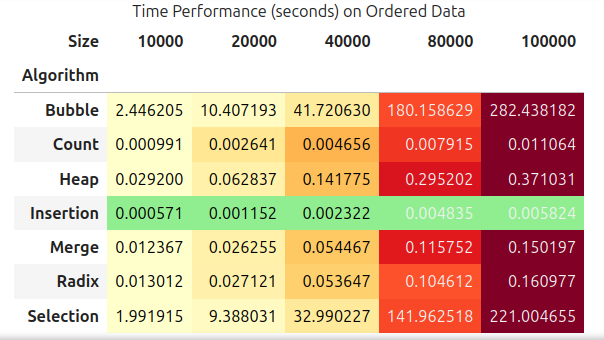
\includegraphics[width=0.6\textwidth]{images/order_table}
  \caption{Tabela Dados Ordeanados}
  \label{fig:Tabela Dados Ordenados}
\end{figure}

\begin{figure}[H]
  \centering
  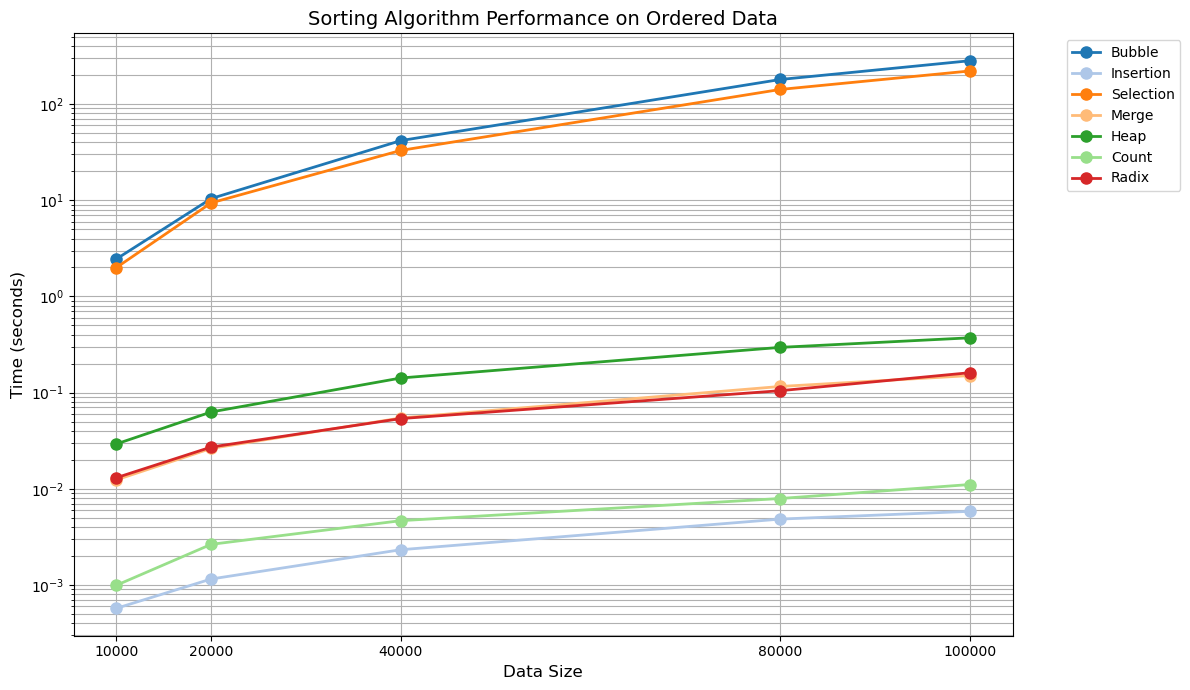
\includegraphics[width=0.6\textwidth]{images/all_algo_order}
  \caption{Gráfico Performance Dados Ordenados em escala Logaritmica}
  \label{fig:Gráfico Performance Dados Ordenados}
\end{figure}

\begin{figure}[H]
  \centering
  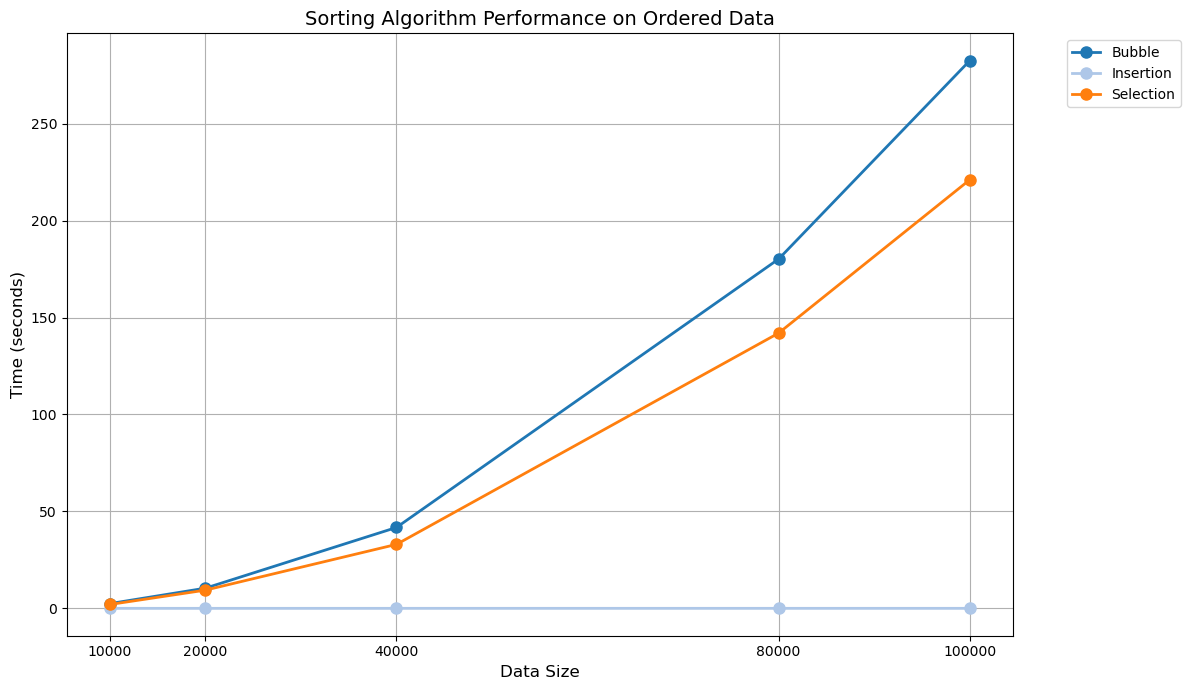
\includegraphics[width=0.6\textwidth]{images/o2_order}
  \caption{Performance Bubble, Insertion e Selection em Dados Ordenados}
  \label{fig:Performance Bubble, Insertion e Selection em Dados Ordenados}
\end{figure}

\begin{figure}[H]
  \centering
  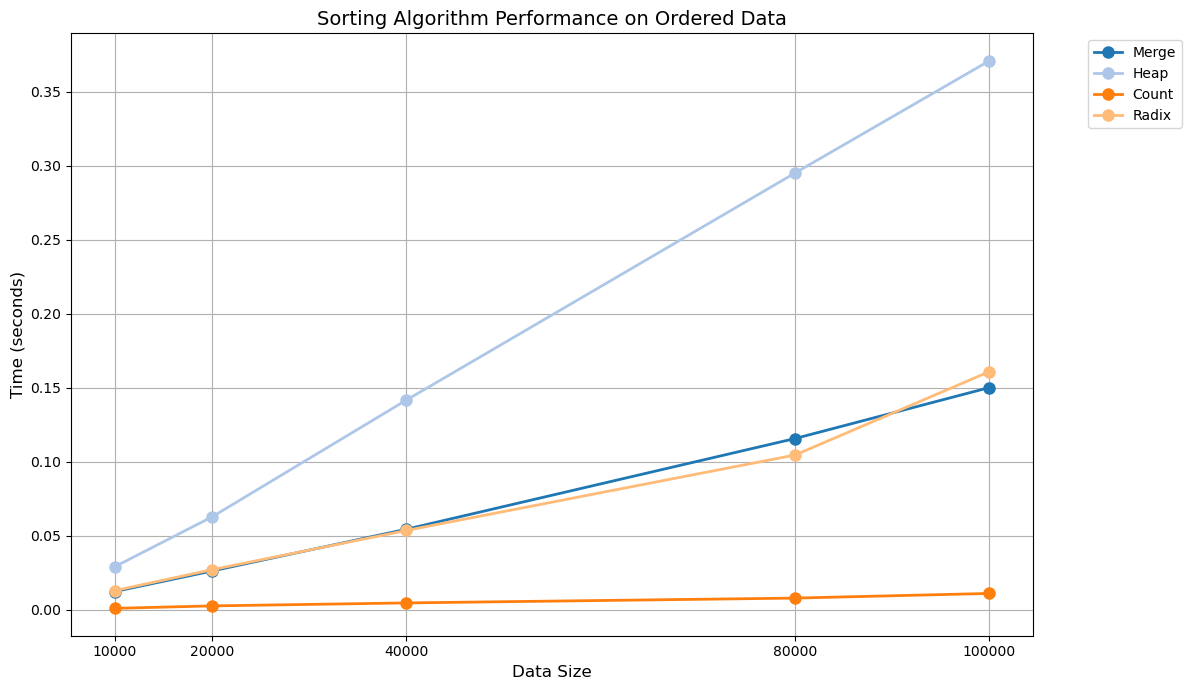
\includegraphics[width=0.6\textwidth]{images/o_order}
  \caption{Performance Restante em Dados Ordenados }
  \label{fig:Gráfico Performance Dados Ordenados}
\end{figure}

\subsection{Analise para Dados Ordenados}
Para os dados Ordenados:
\begin{itemize}
  \item Pior Algorimo: Bubble Sort
  \item Melhor Algoritmo: Insertion Sort
\end{itemize}
Pela analise dos gráficos, observa-se os seguintes comportamentos:
\begin{itemize}
  \item Parabólico: Selection e Bubble. Comportamento esperado 
  \item Logaritmico: Radix e Merge. Esperado para Merge, inesperado para Radix 
  \item Linear: Heap e Insertion. Comportamento Inesperado
\end{itemize}
%%%%%%%%%%%%%%%%%%%%%%%%%%%%%%%%%%%%%%%%%%%%%%%%%%%%%%%%%%%%%%%%%%%%%%%%%%%%%%%%%%%%%%%%%
%%%%%%%%%%%%%%%%%%%%%%%%%%%%%%%%%%%%%%%%%%%%%%%%%%%%%%%%%%%%%%%%%%%%%%%%%%%%%%%%%%%%%%%%%
\section{Resultados para DataSet Inversamente Ordenado}

\begin{figure}[H]
  \centering
  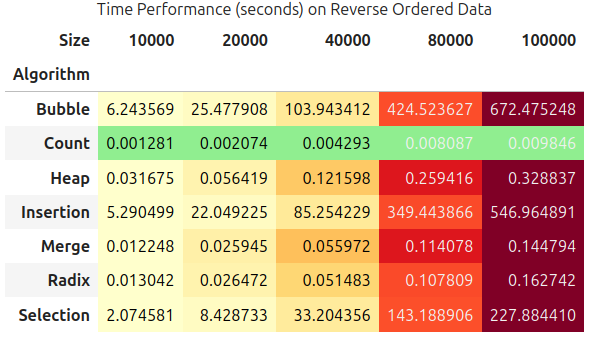
\includegraphics[width=0.6\textwidth]{images/invert_table}
  \caption{Tabela Dados Inversamente Ordenados}
  \label{fig:Tabela Dados Inversamente Ordenados}
\end{figure}

\begin{figure}[H]
  \centering
  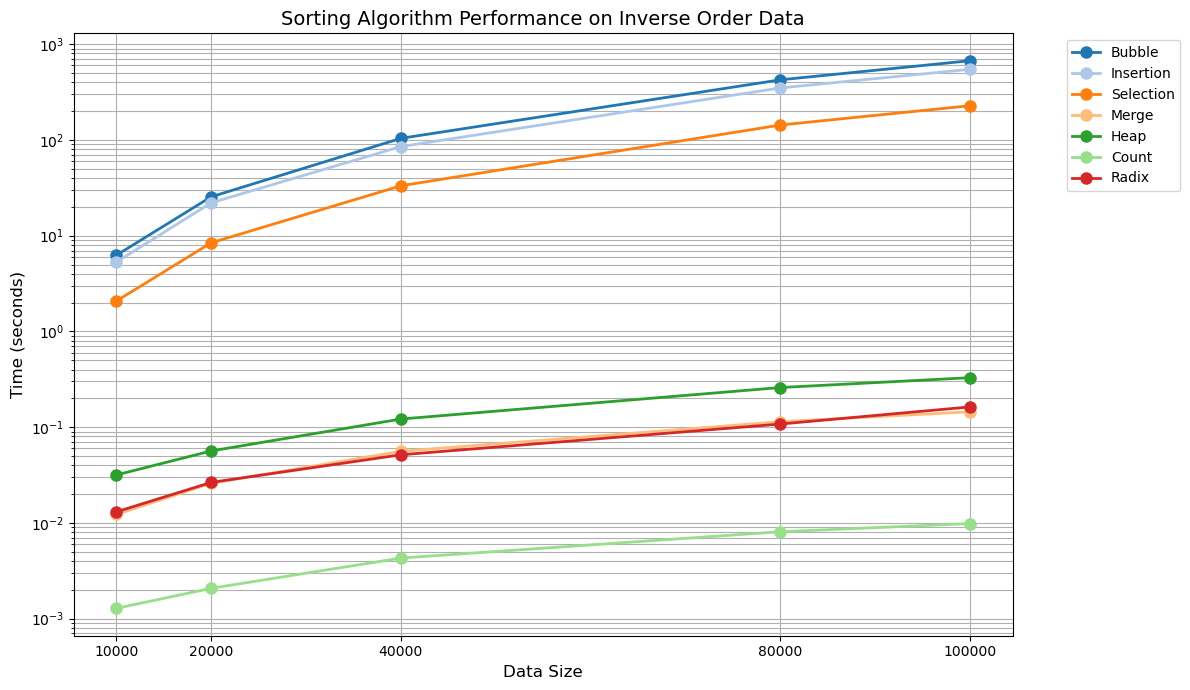
\includegraphics[width=0.6\textwidth]{images/all_algo_inver}
  \caption{Gráfico Performance Dados Inversamente Ordenados em escala Logaritmica}
  \label{fig:Gráfico Performance Dados Inversamente Ordenados}
\end{figure}

\begin{figure}[H]
  \centering
  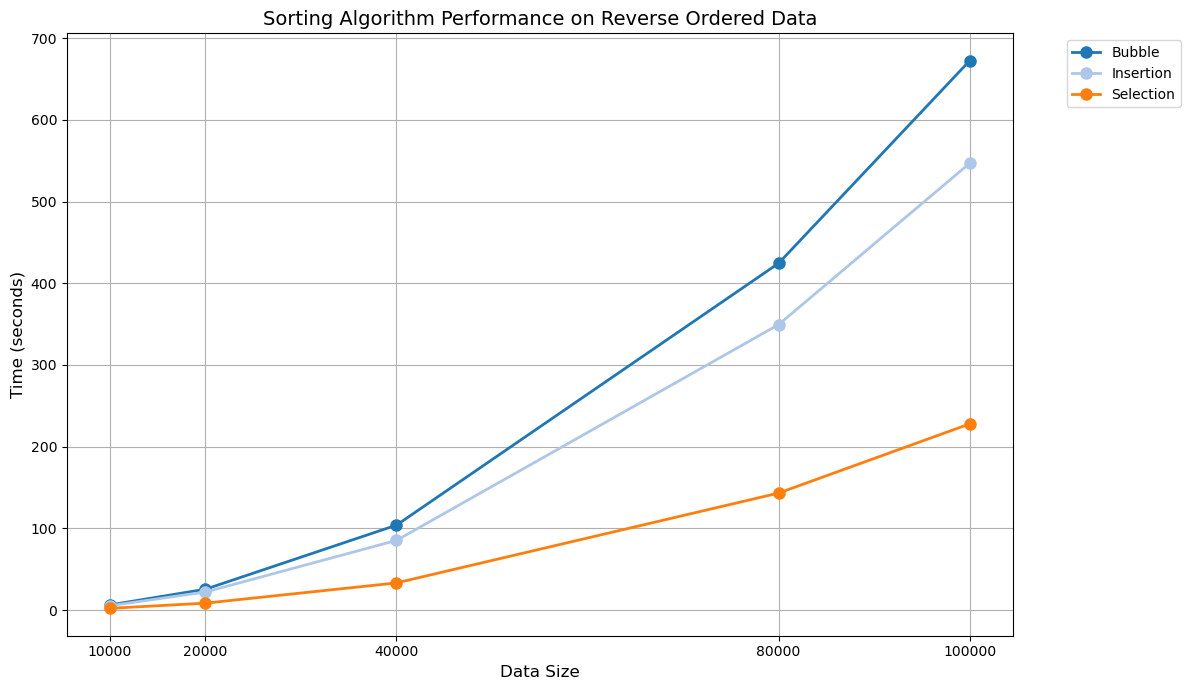
\includegraphics[width=0.6\textwidth]{images/o2_inv}
  \caption{Performance Bubble, Insertion e Selection em Dados Inversamente Ordenados}
  \label{fig:Performance Bubble, Insertion e Selection em Dados Inversamente Ordenados}
\end{figure}

\begin{figure}[H]
  \centering
  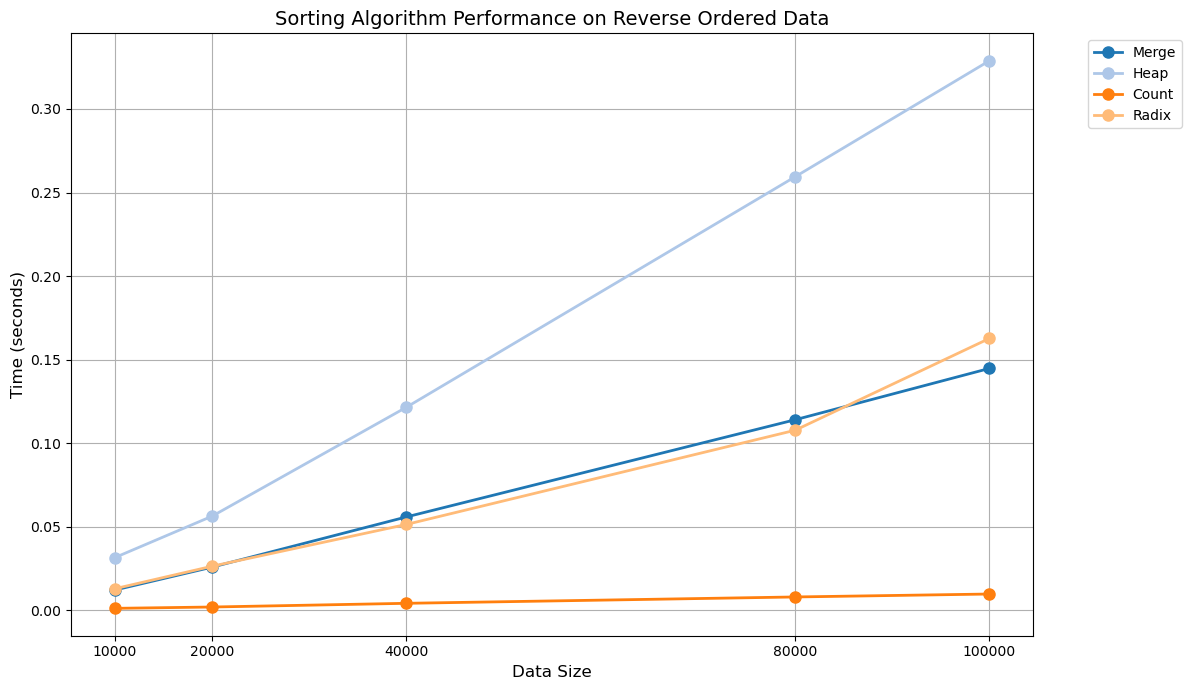
\includegraphics[width=0.6\textwidth]{images/o_inv}
  \caption{Performance Restante em Dados Inversamente Ordenados }
  \label{fig:Gráfico Performance Dados Inversamente Ordenados}
\end{figure}

\subsection{Analise para Dados Inversamente Ordenados}
Para os dados Inversamente Ordenados:
\begin{itemize}
  \item Pior Algorimo: Bubble Sort
  \item Melhor Algoritmo: Count Sort
\end{itemize}
Pela analise dos gráficos, observa-se os seguintes comportamentos:
\begin{itemize}
  \item Parabólico: Selection,  Bubble e Insertion. Comportamento esperado 
  \item Logaritmico: Radix, Merge e Heap. Inesperado para Radix 
  \item Linear: Count. Comportamento Inesperado
\end{itemize}

%%%%%%%%%%%%%%%%%%%%%%%%%%%%%%%%%%%%%%%%%%%%%%%%%%%%%%%%%%%%%%%%%%%%%%%%%%%%%%%%%%%%%%%%%
%%%%%%%%%%%%%%%%%%%%%%%%%%%%%%%%%%%%%%%%%%%%%%%%%%%%%%%%%%%%%%%%%%%%%%%%%%%%%%%%%%%%%%%%%
\section{Resultados para DataSet Aleatoriamente Ordenado}
\begin{figure}[H]
  \centering
  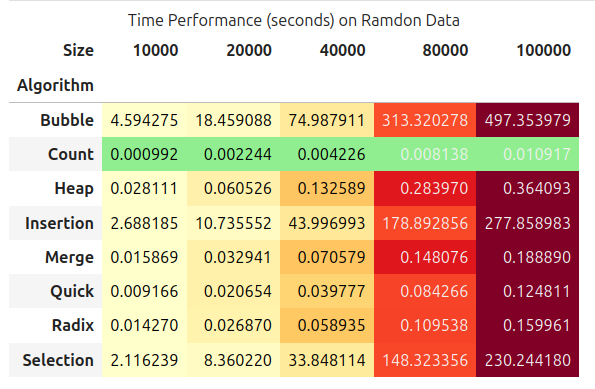
\includegraphics[width=0.6\textwidth]{images/random_table}
  \caption{Tabela Dados Aleatoriamente Ordenados}
  \label{fig:Tabela Dados Aleatoriamente Ordenados}
\end{figure}

\begin{figure}[H]
  \centering
  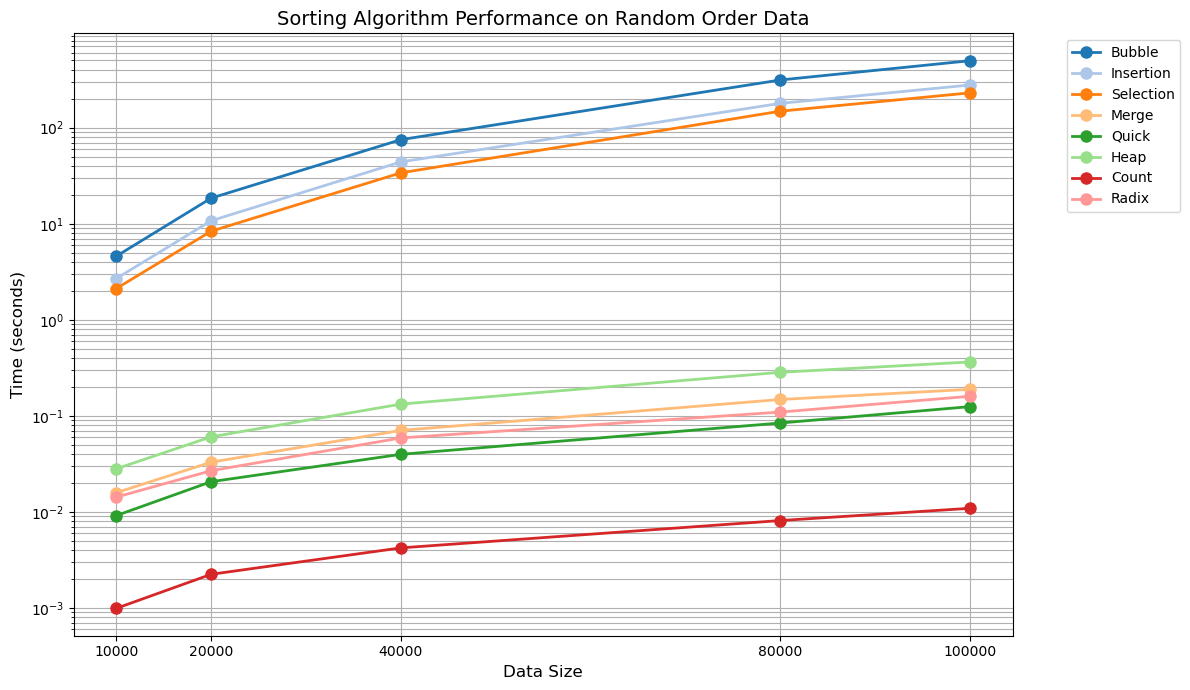
\includegraphics[width=0.6\textwidth]{images/all_algo_rand}
  \caption{Gráfico Performance Dados Aleatoriamente Ordenados em escala Logaritmica}
  \label{fig:Gráfico Performance Dados Aleatoriamente Ordenados}
\end{figure}

\begin{figure}[H]
  \centering
  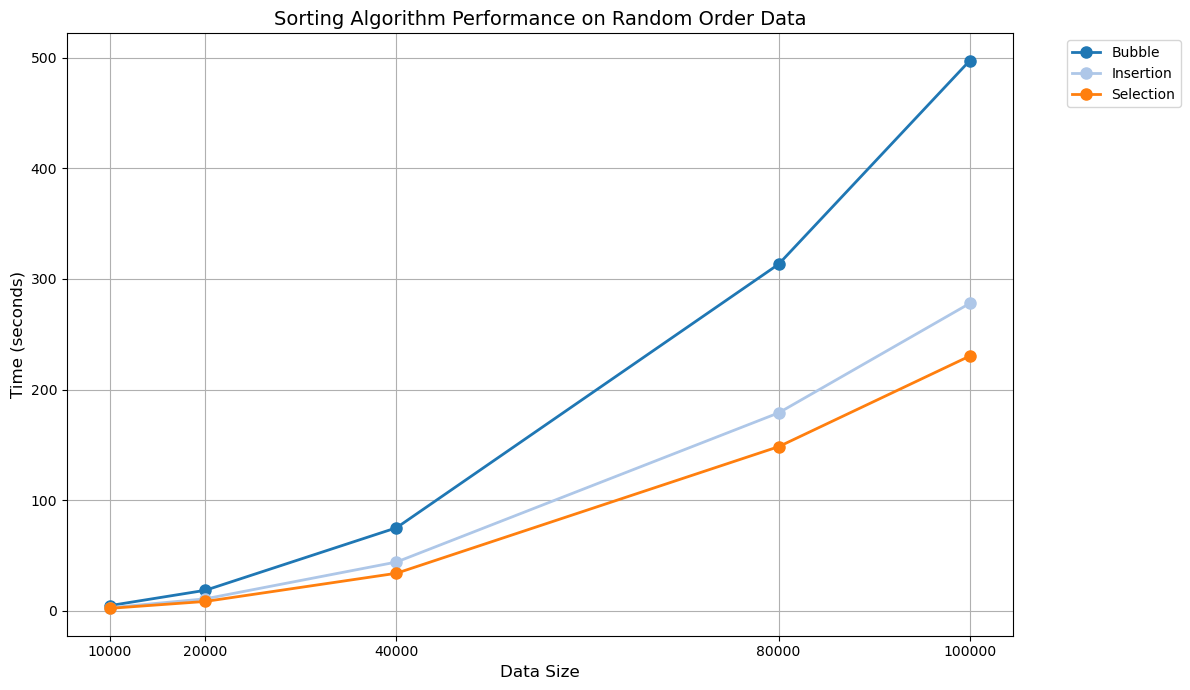
\includegraphics[width=0.6\textwidth]{images/o2_random}
  \caption{Performance Bubble, Insertion e Selection em Dados Aleatoriamente Ordenados}
  \label{fig:Performance Bubble, Insertion e Selection em Dados Aleatoriamente Ordenados}
\end{figure}

\begin{figure}[H]
  \centering
  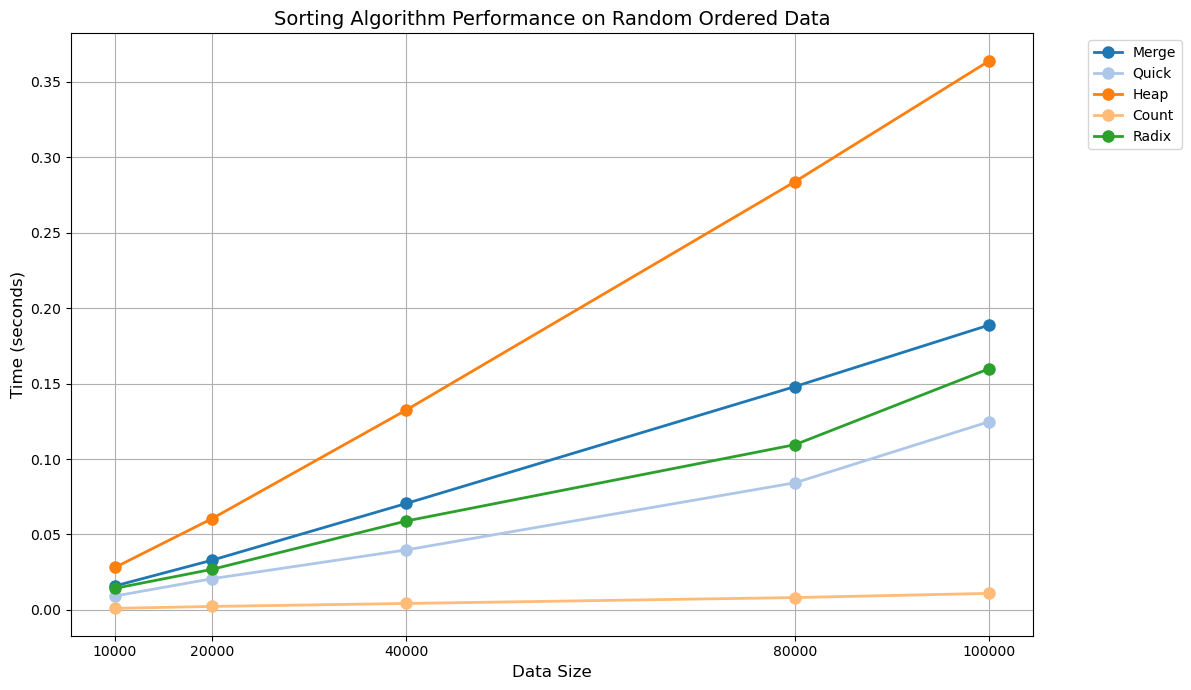
\includegraphics[width=0.6\textwidth]{images/o_random}
  \caption{Performance Restante em Dados Aleatoriamente Ordenados }
  \label{fig:Gráfico Performance Dados Aleatoriamente Ordenados}
\end{figure}

\subsection{Analise para Dados Aleatoriamente Ordenados}
Para os dados Inversamente Aleatoriamente Ordenados:
\begin{itemize}
  \item Pior Algorimo: Bubble Sort
  \item Melhor Algoritmo: Count Sort 
\end{itemize}
Pela analise dos gráficos, observa-se os seguintes comportamentos:
\begin{itemize}
  \item Parabólico: Selection,  Bubble e Insertion. Comportamento esperado 
  \item Logaritmico: Radix, Merge e Quick. Esperado apenas para Merge 
  \item Linear: Count e Heap. Comportamento Inesperado para Heap
\end{itemize}

\chapter{Conclusões}
Um dos comportamentos inesperados para o Radix muito provavelmente vem da implementação do mesmo, que precisa encontrar o máximo dentre os elementos, consequentemente varrendo os mesmos até o final pelo menos uma vez. 
O comportamento dos algotimos também permite concluir que o melhor deles em termos de tempo de execução foi o Counting sort, exceto para o caso dos já ordenados, que foi o Insertion Sort, comportamento esperado do mesmo visto que ele apenas compara uma vez cada elemento, que por conta de estarem na ordem correta não precisam ser comparados com os anteriores, o que acarreta no comportamento linear.

Em conclusão, o projeto permitiu um aprofundamento no conhecimento dos diversos algoritmos de ordenação bem como seu funcionamento interno e requisitos de sistema. 
Uma futura pesquisa poderia pegar a base do projeto porém além de realizar as comparações de tempo dentro da mesma linguagem, realizar a implementação dos memsmos algoritmos em outras linguagens e então comparar o tempo etre elas.

\begin{appendices}
  \chapter{Fonte}
  Todo o código fonte e os materias utilizados para produção do relatório se encontram no repositório abaixo:

  \url{https://github.com/sheeptraveler/sorting\_algorithms\_comparison\_python}
\end{appendices}



%%%%%%%%%%%%%%%%%%%%%%%%%%%%%%%%%%%%%%%%%%%%%%%%%%%%%%%%%%%%%%%%%%%%%%%%%%%%%%%%%
%% Source defintions
%%%%%%%%%%%%%%%%%%%%%%%%%%%%%%%%%%%%%%%%%%%%%%%%%%%%%%%%%%%%%%%%%%%%%%%%%%%%%%%%%
% When no use outcomment
%\bibliographystyle{alpha}

\renewcommand\bibname{References}
\bibliography{base/sources}


%%%%%%%%%%%%%%%%%%%%%%%%%%%%%%%%%%%%%%%%%%%%%%%%%%%%%%%%%%%%%%%%%%%%%%%%%%%%%%%%%
%% Inserting the appendix
%%%%%%%%%%%%%%%%%%%%%%%%%%%%%%%%%%%%%%%%%%%%%%%%%%%%%%%%%%%%%%%%%%%%%%%%%%%%%%%%%
% When no use outcomment
%\include{appendix/appendix}
\end{document}*/***********************************************************************8	
